% !TEX root=/home/tavant/these/manuscript/src/manuscript.tex


\section{Polytropic electrons in the presence of \acs{SEE}}
\label{sec-PIC_poly}

The sheath model developed in \cref{ch-3} uses a polytropic state law for the electrons instead of the usual isothermal approximation.
Indeed, the results of the  \ac{1D} \ac{PIC} simulations presented a polytropic evolution of the electrons.
This model successfully reproduced the sheath characteristics  when no secondary electron emission was modeled (fully absorbing walls).
Before adapting this sheath model to the case with \ac{SEE}, we need to validate the polytropic hypothesis in the presence of \ac{SEE}.


\subsection{Determination of the polytropic index from PIC simulations} \label{subsec-fluid_see_polyfit}


The \ac{2D} \ac{PIC} simulation is described in \cref{ch-2}, but we recall here the main parameters.
The bidimensional domain lengths $2\,\centi\meter$ in the radial direction, and $0.25\,\centi\meter$ in the azimuthal direction.
A radial magnetic field $B=200\,$G and an axial electric field $E=20\,\kilo\volt\per\meter$ are applied.
The mean plasma density is $n_e = \sn{3}{17}\,\meter^{-3}$.
The radial direction is closed by grounded wall, but we model the electron induced electron emission from the wall.
The model used is described in \cref{sec-seemodel}, using the parameters of \cref{tab-tabe_parameters_see}.
In addition, the axial convection is modeled using Lafleur's model of convection, as discussed in \cref{sec-reinjectionnoise}.

\Cref{fig-2DneTe} shows the electron density and the electron temperature obtained at the end of the simulation ( $t=10\,\micro\second$) in the case $\crover=200\,\volt$.
We can see the azimuthal instability in both $n_e$ and $\Te$.
However, these azimuthal oscillations will be averaged in the following development. 

% \renewcommand\subfigurewidth{0.5\textwidth}

\begin{figure}[!htb]
  \centering
  \begin{tabular}{@{} c c}
    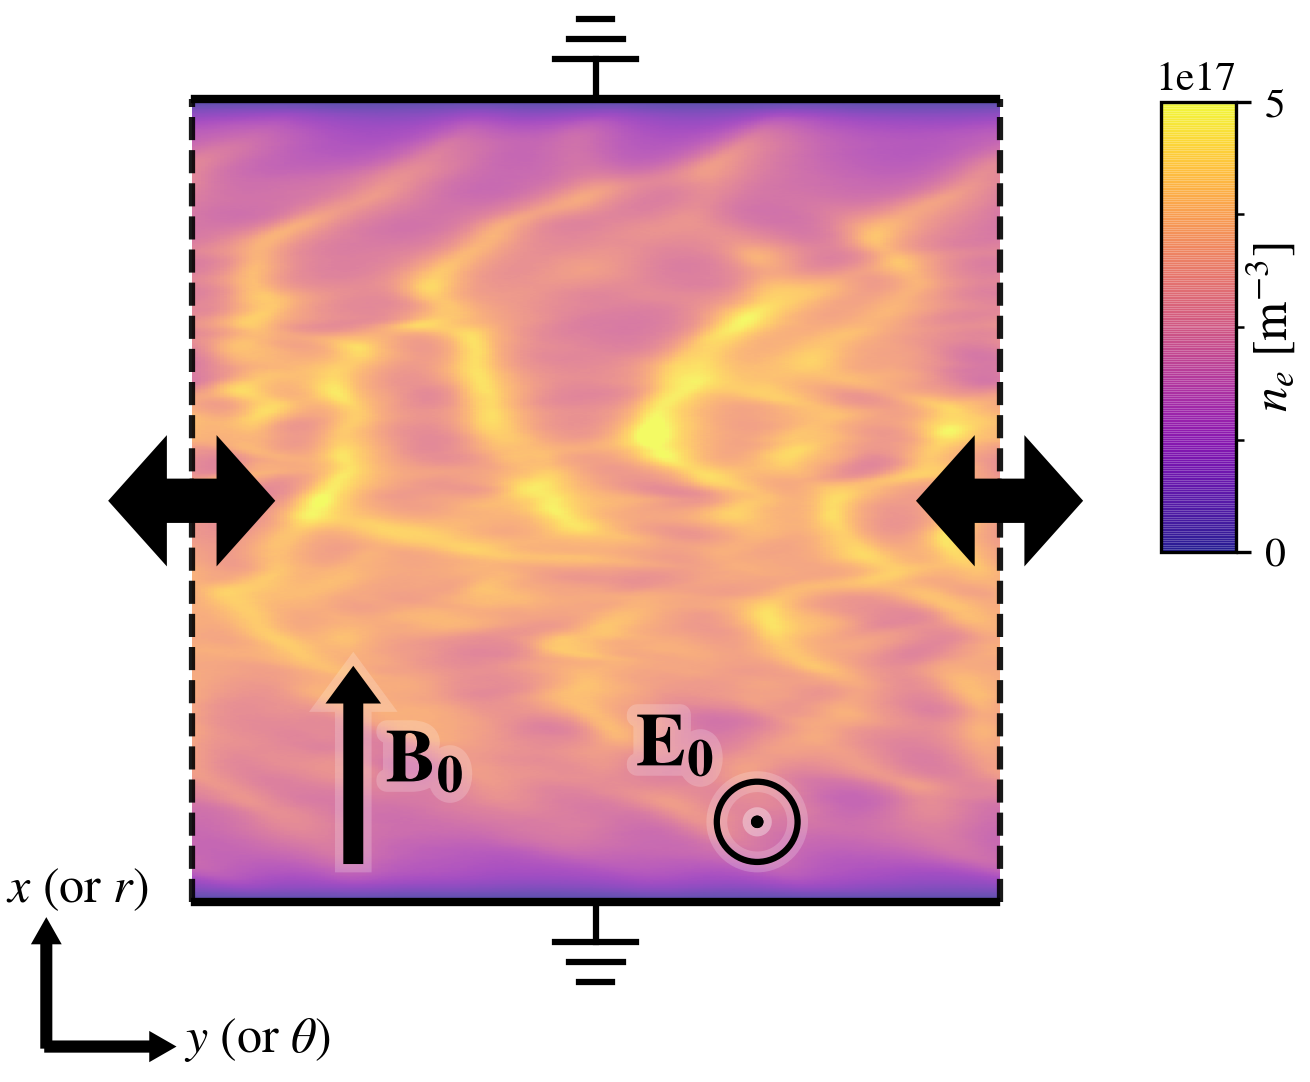
\includegraphics[width=0.49\textwidth]{2D_ne_SEE200} &
    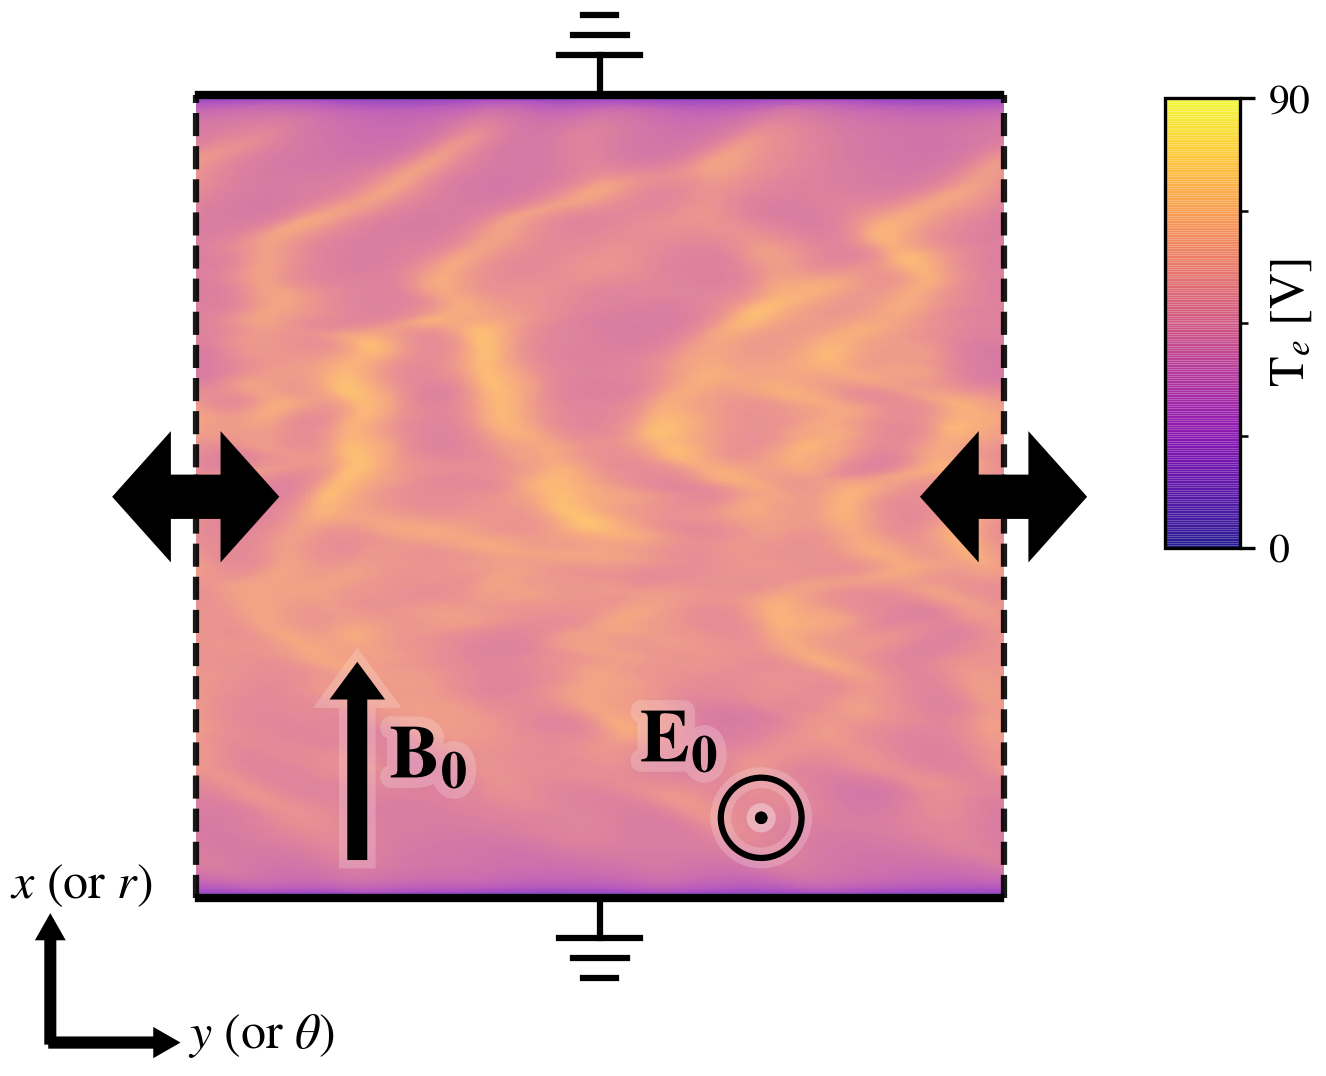
\includegraphics[width=0.49\textwidth]{2D_Te_SEE200} \\
  \end{tabular}
  \caption{Maps of the (left) electron density $n_e$ and (right) electron temperature $T_e$ at $t=10\,\micro\second$ in the \acs{2D} simulation domain with $\crover=200\,\volt$.}
  \label{fig-2DneTe}
\end{figure}



As previously done in \cref{ch-3}, we use the mean values of the electron density $n_e$ and the electron pressure $ p_e = e n_e T_e$ to find the value of the polytropic index.
\Cref{fig-radial_profiles_see} shows the radial profiles of the electron density and temperature for different values of the cross-over energy $\crover$.
The three values of $\crover$ used are representative of the behaviors observed.
Indeed, $\crover=200\,\volt$ and $\crover=50\,\volt$ correspond to the upper and lower limits of regime {\bf III}, corresponding to low emission rate $\rate$, while regime {\bf I} corresponds to the case $\crover=10\,\volt$.
Regime {\bf II} is not presented, as the oscillating nature of the sheath is not taken into account by the stationary sheath model developed here. 


\begin{figure}[!htb]
  \centering
  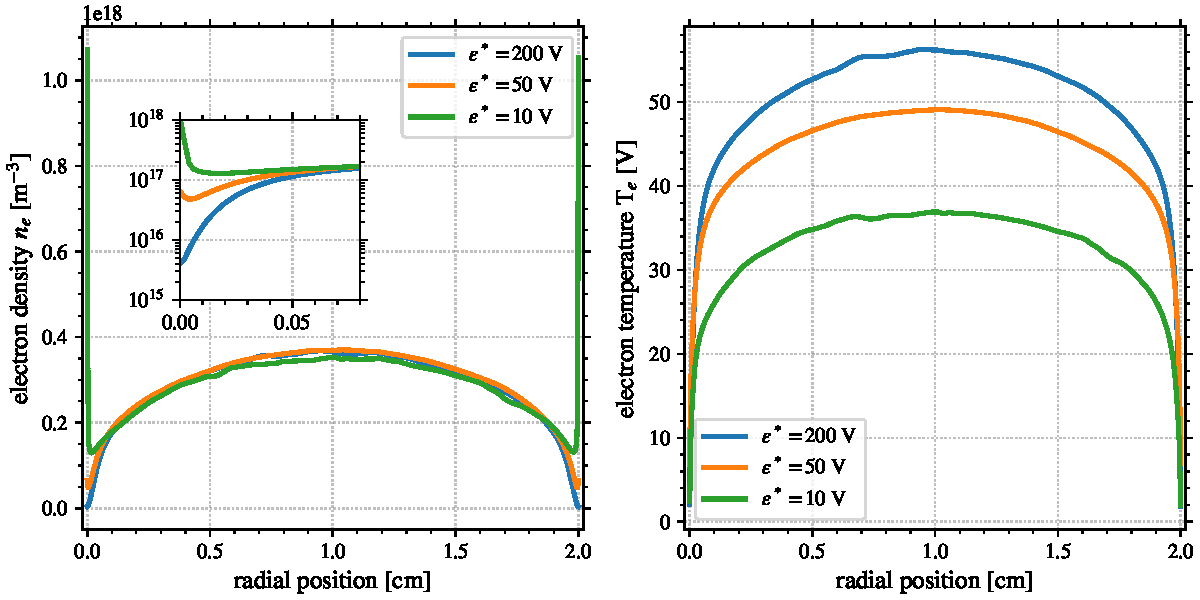
\includegraphics[width=\textwidth]{ne_Te_profiles.pdf}
  \caption{Radial profiles of (left) the electron density and (right) the electron temperature, for different values of $\crover$. The variables are averaged over the azimuthal direction and in time between $t=5\,\micro\second$ and $t=10\,\micro\second$.  }
  \label{fig-radial_profiles_see}
\end{figure}

We see in \cref{fig-radial_profiles_see} that the electron temperature presents a monotonic profile for all the values of $\crover$.
However, for low value of $\crover$ the electron density is not monotonic, but instead presents an increase close to the wall.
This is clearly visible in \cref{fig-log_pe-ne}, which presents the electron pressure $p_e$ as a function of the electron density $n_e$, in log scale and normalized by the values at the center.
We see that close to the wall, where the electron pressure is the lowest, the curves present an inversion, in contrast with the case without electron emission seen in \cref{fig-polyFit}.
Otherwise in the rest of the domain, the curves are almost linear, corresponding to a polytropic state law.

\begin{figure}[!htb]
  \centering
  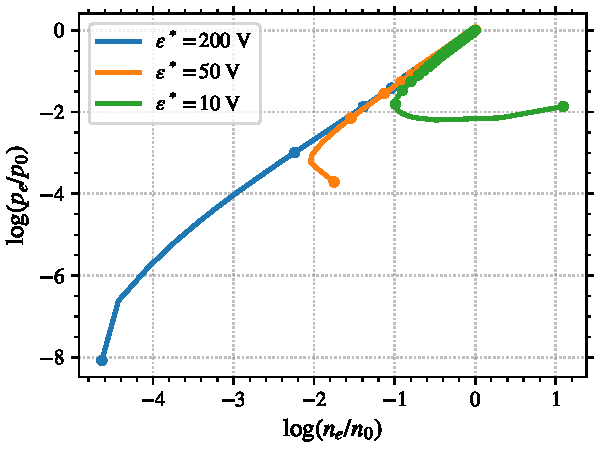
\includegraphics[width=\defaultwidth]{SEE_polytropic_presheath_and_sheath.pdf}
  \caption{Electron pressure as a function of the electron density normalized by the center variable, in log scale. The data corresponds to the same as \cref{fig-radial_profiles_see}. Markers are used every 10 cells (corresponding to around one Debye length $\lde$)}
  \label{fig-log_pe-ne}
\end{figure}

The steep increase of the electron density is due to the cold secondary electron population, that resides next to the wall before being accelerated through the sheath toward the plasma.
In addition, under the \ac{SCL} regime ($\crover = 10\,\volt$) the plasma potential presents a local minimum close to the wall, that reflect secondary electrons back to the wall.
However, we see that it appends only over the last Debye length $\lde$.
Consequently, in the following we neglect this increase of the electron density.

We determine the value of the polytropic index $\gamma$ from the \ac{PIC} simulations with a least mean square linear regression.
The results of the regressions are displayed in \cref{fig-polyfit_see}, and the polytropic index obtained are summarized in \cref{tab-summarygamma}.


\begin{figure}[!htb]
  \centering
  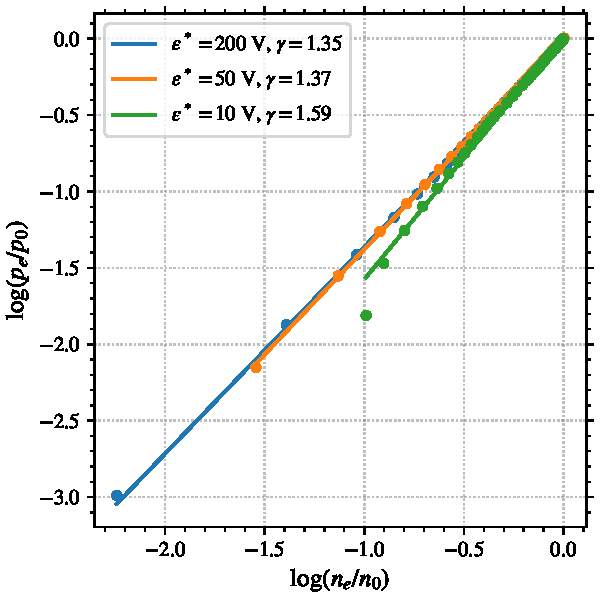
\includegraphics[width=\defaultwidth]{SEE_polyfit}
  \caption{Polytropic linear regression for different values of $\crover$, in the same conditions that \cref{fig-log_pe-ne}, but the last 10 cells near the wall are removed. The values of $\gamma$ fitted on the \acs{PIC} simulation data are given in the legend.}
  \label{fig-polyfit_see}
\end{figure}

\begin{table}[!htb]
\ra{1.3}
  \centering
  \caption{Polytropic index extracted from the \acs{2D}  \acs{PIC} simulations}
  \label{tab-summarygamma}
  \begin{tabular}{@{}r l@{}} \toprule
  Crossover energy $\crover$ & Polytropic index $\gamma$ \\ \midrule
  200 V & 1.35 \\
  50 V & 1.37 \\
  10 V & 1.59 \\
  \bottomrule
  \end{tabular}
\end{table}


We can see that the value of $\gamma$ does not evolve significantly in regime {\bf III}, as it evolves from $\gamma=1.35$  to $1.37$ when $\crover$ vary from $200$ to $50\,\volt$.
For $\crover=10\,\volt$, the value of the polytropic index in the linear stage is $\gamma=1.59$, which is not so different from the values in regime {\bf III}.
However, we will see later that during the regime {\bf I}, the characteristics of the sheath is not affected by the polytropic index. 
Consequently, we suppose in the following that the polytropic index in the \ac{PIC} simulation with secondary electron emission is constant and equals $\gamma=1.36$ for all values of $\crover$.
It will be used in the next sections to compare the \ac{PIC} results with a fluid model of the sheath.

\subsection{Evolution of the forward electron population} \label{subsec-EVDF_see_polyfit}

The electron density $n_e$ and  temperature $\Te$ showed in \cref{subsec-fluid_see_polyfit} (\cref{fig-radial_profiles_see,fig-log_pe-ne,fig-polyfit_see,}) include both the primary electrons going toward the wall and the secondary electron emitted from the wall.
However, the \ac{SEE} rate only depends on the primary electron reaching the wall.
In order to separate the two populations, we use the \ac{EVDF} obtained in the simulations.
\Cref{fig-evdf_epsstar} presents the \ac{EVDF} measured at the center of the simulation domain. 
We see that the \ac{EVDF} presents similar profiles for the three cases, except for the mean energy that decreases with increasing value of $\crover$.
\begin{figure}[!hbt]
  \centering
  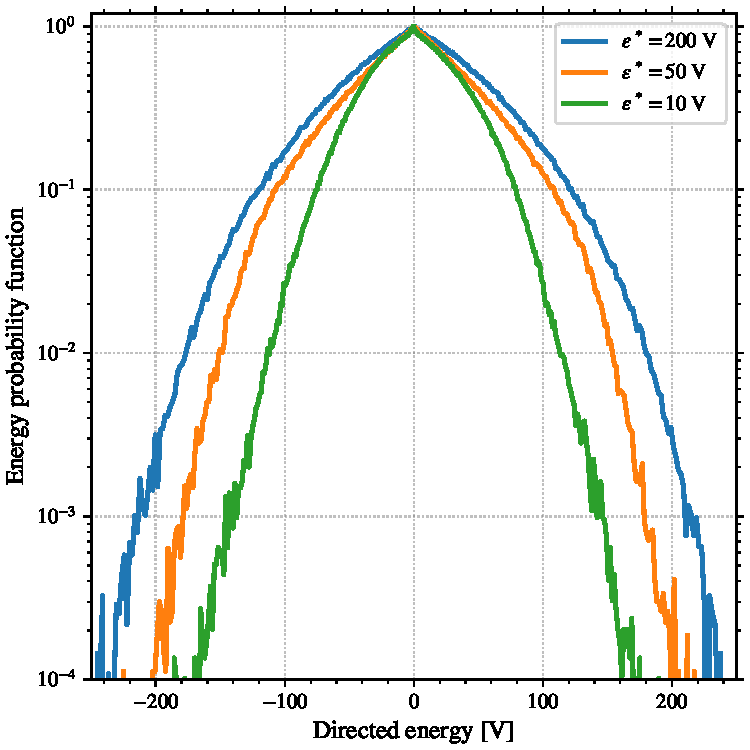
\includegraphics[width=\defaultwidth]{EVDF_Bulk.pdf}
  \caption{Electron velocity distribution function at the center of the simulation, under the same parameters than the cases in \cref{fig-log_pe-ne,fig-polyfit_see}. The sign of the energy corresponds to the direction of the movement.}
  \label{fig-evdf_epsstar}
\end{figure}

We note that no beam is present here, even in the case of very large electron emission at $\crover=10\,\volt$, in contrast with observations of \ac{1D} PIC simulations \citep{sydorenko2006b,sydorenko2007}, but in agreement with the \ac{2D} results of \citet{heron2013}.
This shows that the instability, self-consistently modeled in the \ac{2D} simulations, thermalizes the secondary electron population.

Using the solution of the stationary Vlasov equation \cref{eq-sol}, we compute the evolution of the density and temperature of the primary electron population going toward the wall through the plasma potential $\phi$ 
\begin{equation} \label{eq-vlasovch4}
  \begin{dcases}
    f(\phi, v_e) = f \lp 0, \sqrt{v_e^2 + \frac{2 e}{m_e} \phi} \rp \\
    n_e(\phi) = \int_0^{+\infty} f(\phi, v_e) dv_e \\
    p_e(\phi) = \frac{m_e}{e} \int_0^{+\infty} v_e^2 f(\phi, v_e) dv_e \\
  \end{dcases}
\end{equation}
The results obtained by the system of equations (\ref{eq-vlasovch4}) are shown for the three cases in \cref{fig-evdf_polyfit}.
We see that the forward electron population follows a polytropic law.
For $\crover= 200$ and $50\,\volt$, the corresponding polytropic index is $\gamma=1.28$, while for $\crover= 10\,\volt$ we measure $\gamma=1.35$.

\begin{figure}[hbt]
  \centering
  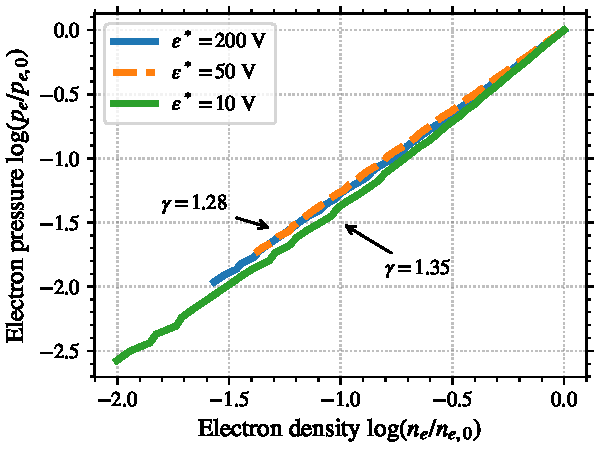
\includegraphics[width=\defaultwidth]{polyfit_evdf}
  \caption{Electron pressure as a function of the electron density in log scale of the forward (primary) electron population using the stationary Vlasov equation \cref{eq-vlasovch4} for (blue) $\crover=200\,\volt$, (dashed orange) $\crover=50\,\volt$, and (green) $\crover=10\,\volt$.}
  \label{fig-evdf_polyfit}
\end{figure}

The fact that the polytropic index of the primary electron is lower than that of the total electron population ($\gamma=1.28$ versus $1.36$) means that the electron temperature of the primary electron population going toward the wall decreases more slowly than the total electron pressure.
This is certainly due to the partial absorption and emission of secondary electrons at the wall, injected at $\Tsee=2\,\volt$ which is small compared to $\Te$.
Hence, we can expect that the emission rate $\rate$, which directly depends on the forward electron population, be better described with the polytropic index $\gamma=1.28$, computed in \cref{fig-evdf_polyfit}, than with $\gamma=1.36$ from \cref{subsec-fluid_see_polyfit}.

